在未特殊写明单位的情况下,本节的默认长度单位是mm,扭矩单位是$\mathrm{N}\cdot \mathrm{mm}$,转速的单位是$\mathrm{r}\cdot \mathrm{min^{-1}}$,力的单位是N。
\subsection{草图准备}
\subsubsection{选定联轴器类型}
对于连接电动机和减速器高速轴的联轴器,为了减小启动转矩,其联轴器类型应具有较小的转动惯量和较好的减震性能,故采用弹性柱销联轴器,对于低速轴和工作机相连的联轴器,因其转速较低,转矩较大,考虑到本设计安装时不易保证同心度,采用具有良好补偿位移偏差的凸缘联轴器。
\subsubsection{确定滚动轴承类型}
对于高速级斜齿圆柱齿轮传动,因有轴向力相比于径向力小很多,选择深沟球轴承;低速级也同样采用圆锥滚子轴承。
\subsubsection{确定滚动轴承的润滑和密封方式}
由前面计算可知高速级齿轮线速度 ,低速级齿轮线速度 ,故滚动轴承采用L-AN68润滑油润滑,并在轴上安装挡油板。考虑减速器工作环境有尘,轴颈圆周速度 ,故采用唇型圈密封。
\subsubsection{确定轴承端盖的结构形式}
凸缘式轴承端盖调整轴承间隙比较方便,密封性能也好,故选用凸缘式轴承端盖,采用铸铁铸造成型。
\subsubsection{确定减速器机体的结构方案}
考虑工艺性能、材料消耗和制造成本,选用剖分式机体,铸铁材料铸造成型。结构示例图如下图所示:
\begin{figure}[H]
	\begin{center}
		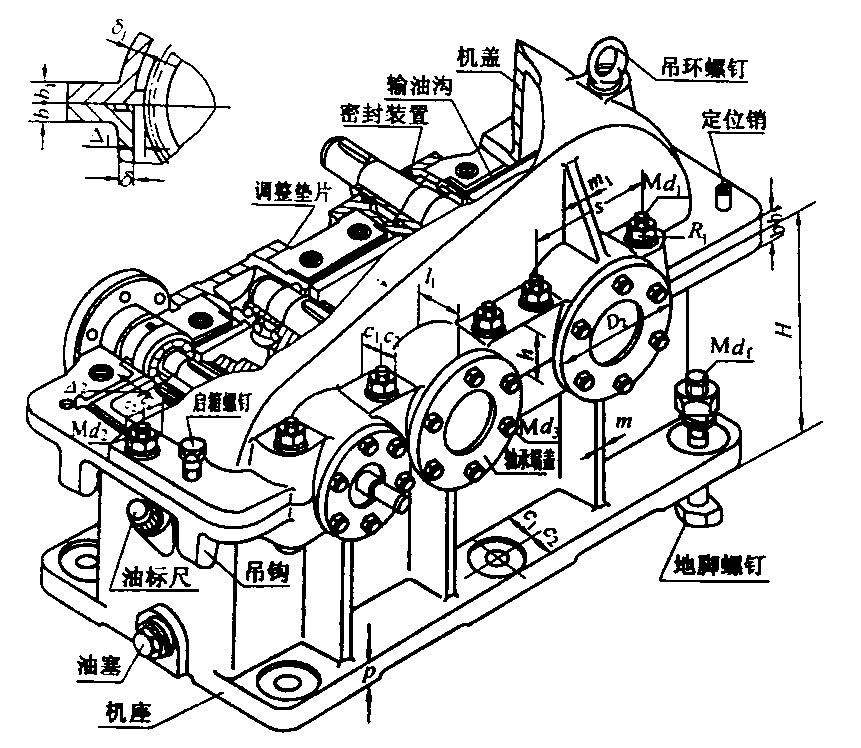
\includegraphics{pic/1.png}
		\caption{减速器机体结构示意}
	\end{center}
\end{figure}
\par 与机体有关零件的结构尺寸见下表:
\begin{table}[H]
	\caption{机体零件尺寸}
	\begin{center}
		\begin{tabular}{cccc}
			\toprule
			名称 & 符号	& 尺寸关系 & 尺寸大小 \\
			\midrule
			基座壁厚 & $\delta$ & $0.025a+3\geq 8$ & 8 \\
			机盖壁厚 & $\delta_1$ & $0.02a+3\geq 8$ & 8 \\
			机座凸缘厚度 & $b$ & $1.5\delta$ & 12 \\
			机盖凸缘厚度 & $b_1$ & $1.5\delta_1$ & 12 \\
			机座底凸缘厚度 & $p$ & $2.5\delta$ & 20 \\
			地脚螺钉直径 & $d_f$ & $0.036a+12$ & 16 \\
			地脚螺钉数目 & $n$ & $n=6$ & 6 \\
			轴承旁连接螺栓直径 & $d_1$ & $0.75d_f$ &M12\\
			机盖与机座连接螺栓直径 & $d_2$ & $(0.5\sim 0.6) d_f$ &M10\\
			轴承端盖螺栓直径 & $d_3$ & $(0.4\sim 0.5)d_f$ &M8\\
			窥视孔盖螺栓直径 & $d_4$ & $(0.3\sim 0.4)d_f$ &M6\\
			定位销直径 & $d$ & $(0.7\sim 0.8)d_2$ & 8\\
			$d_f$、$d_1$、$d_2$至外壁距离 & $c_1$ & —— & 22\\
			$d_f$、$d_2$至凸缘距离 & $c_2$ & —— & 20\\	
			轴承旁凸台半径& $R_1$ & $c_2$ & 20 \\
			凸台高度 & $H$ & 根据低速轴的轴承外径确定 & 40\\
			外机壁至轴承座端面距离 & $l_1$ & $c_1+c_2+(5\sim 8)$ & 48\\
			内机壁至轴承座端面距离 & $l_2$ & $\delta+c_1+c_2+(5\sim 8)$ & 56\\
			大齿轮顶圆与内机壁距离 & $\Delta_1$ & $>1.2\delta$ & 10\\
			齿轮端面与内机壁距离 & $\Delta_2$ & $\geq \delta$ & 10\\
			机盖、机座肋厚 & $m_1$、$m$ & $m_1\approx0.85\delta_1$,$m\approx0.85\delta$ &7\\
			轴承端盖外径 & $D_2$ & 轴承座孔径$+(5\sim 5.5)d_3$ & 92,132\\
			轴承端盖凸缘厚度 & $e$ & $\left(1\sim 1.2\right)d_3$ & 8 \\
			轴承旁连接螺栓距离 & $s$ & $s\approx D_2$ & 视具体轴承而定\\
			\bottomrule
		\end{tabular}
	\end{center}
\end{table}